\documentclass[micros_g1_main.tex]{subfiles}
\begin{document}
\section{Ejercicio 2}

A continuación se presenta una foto del microcontrolador corriendo el programa Blink. 
	\begin{figure}[H]
		\centering
		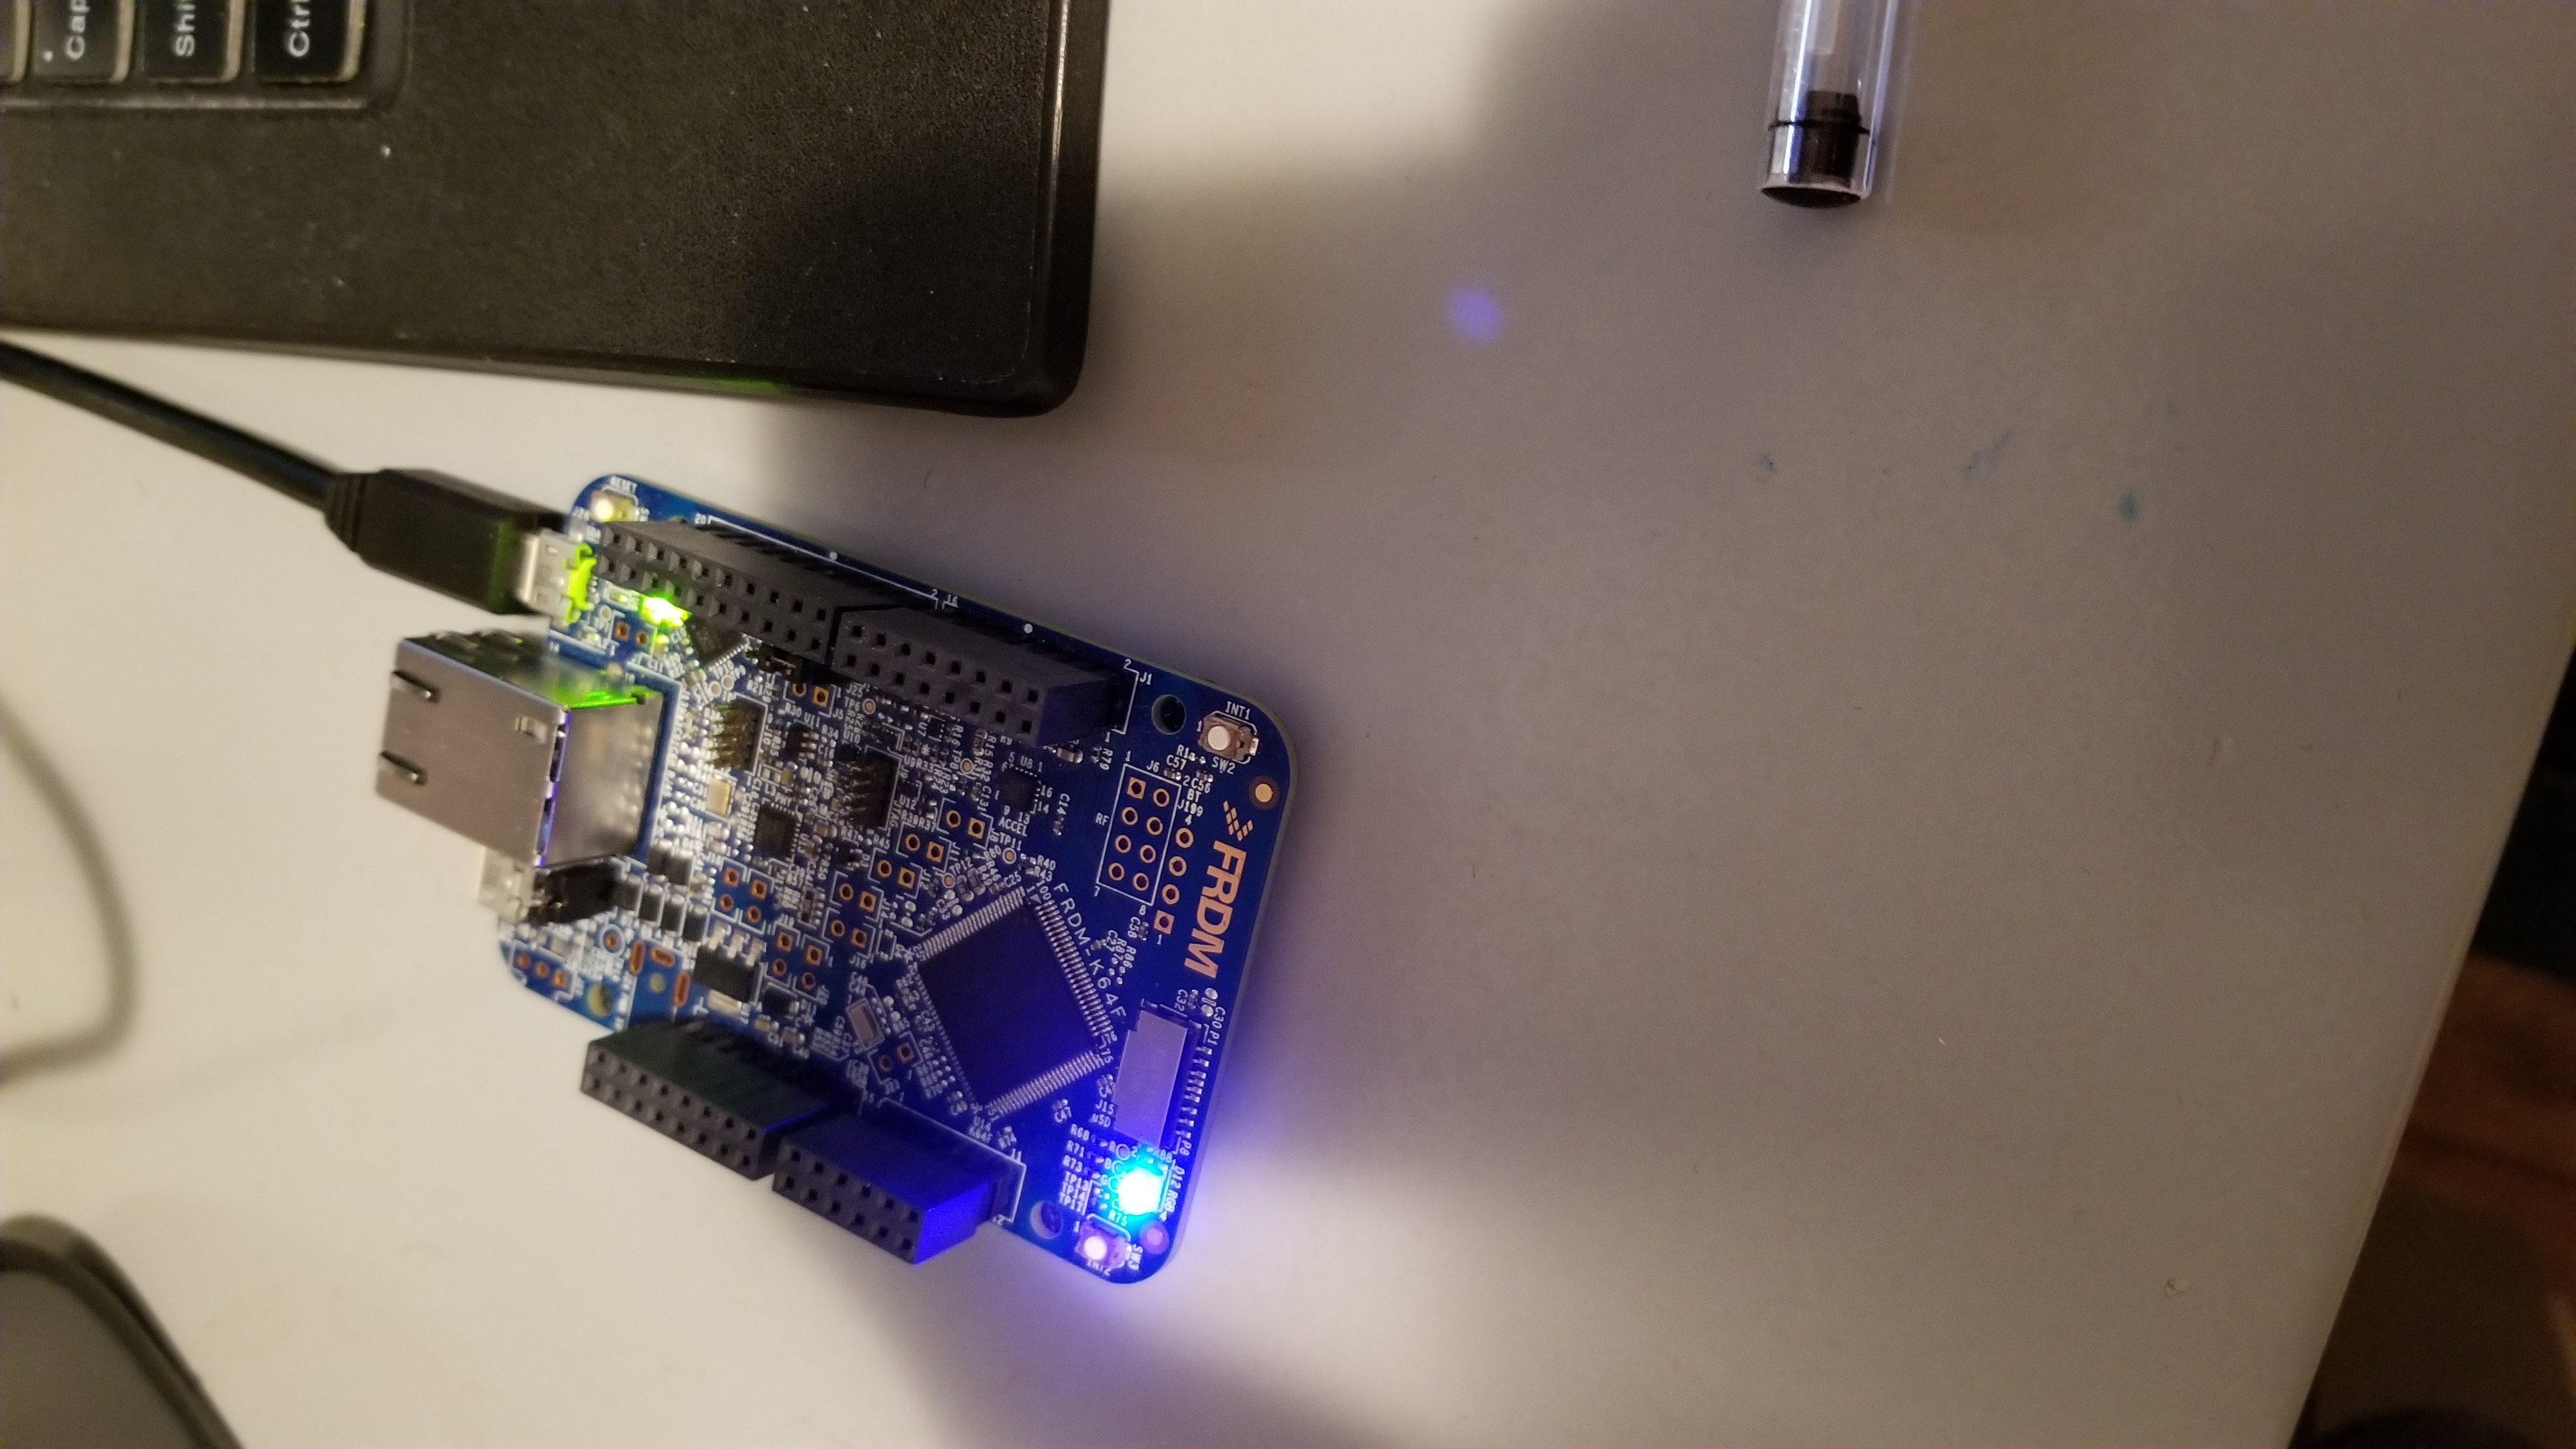
\includegraphics[width=0.45\textwidth]{images/blink_blue.jpg}
		\caption{Corriendo el programa Blink} \label{fig:cct}
	\end{figure}

\subsection{Ítem f}
Se observa que al correr el programa con un nivel de optimización de Optimize Most, el compilador saltea las instrucciones que considera redundantes, en particular en el programa Blink, ignora las iteraciones de la función de delay ya que esta función comprende un while en el que únicamente se incrementa una variable que nunca se utiliza. De esta manera, al ignorar la línea de delay, el compilador estaría optimizando el programa al eliminar código redundante, que en nuestro caso particular afecta al funcionamiento general del mismo. 

\end{document}
